\PassOptionsToPackage{unicode=true}{hyperref} % options for packages loaded elsewhere
\PassOptionsToPackage{hyphens}{url}
%
\documentclass[10pt,xcolor=table,color={dvipsnames,usenames},ignorenonframetext,usepdftitle=false,french]{beamer}
\setbeamertemplate{caption}[numbered]
\setbeamertemplate{caption label separator}{: }
\setbeamercolor{caption name}{fg=normal text.fg}
\beamertemplatenavigationsymbolsempty
\usepackage{caption}
\captionsetup{skip=0pt,belowskip=0pt}
%\setlength\abovecaptionskip{-15pt}
\usepackage{lmodern}
\usepackage{amssymb,amsmath,mathtools,multirow}
\usepackage{float,hhline}
\usepackage{tikz}
\usepackage{mathtools}
\usepackage{ifxetex,ifluatex}
\usepackage{fixltx2e} % provides \textsubscript
\ifnum 0\ifxetex 1\fi\ifluatex 1\fi=0 % if pdftex
  \usepackage[T1]{fontenc}
  \usepackage[utf8]{inputenc}
  \usepackage{textcomp} % provides euro and other symbols
\else % if luatex or xelatex
  \usepackage{unicode-math}
  \defaultfontfeatures{Ligatures=TeX,Scale=MatchLowercase}
\fi
\usetheme[coding=utf8,language=french,
,titlepagelogo=img/logobeamer.png
]{TorinoTh}
% use upquote if available, for straight quotes in verbatim environments
\IfFileExists{upquote.sty}{\usepackage{upquote}}{}
% use microtype if available
\IfFileExists{microtype.sty}{%
\usepackage[]{microtype}
\UseMicrotypeSet[protrusion]{basicmath} % disable protrusion for tt fonts
}{}
\IfFileExists{parskip.sty}{%
\usepackage{parskip}
}{% else
\setlength{\parindent}{0pt}
\setlength{\parskip}{6pt plus 2pt minus 1pt}
}
\usepackage{hyperref}
\hypersetup{
            pdfauthor={Alain Quartier-la-Tente},
            pdfborder={0 0 0},
            breaklinks=true}
\urlstyle{same}  % don't use monospace font for urls
\newif\ifbibliography
\newlength{\cslhangindent}
\setlength{\cslhangindent}{1.5em}
\newlength{\csllabelwidth}
\setlength{\csllabelwidth}{3em}
\newenvironment{CSLReferences}[2] % #1 hanging-ident, #2 entry spacing
 {% don't indent paragraphs
  \setlength{\parindent}{0pt}
  % turn on hanging indent if param 1 is 1
  \ifodd #1 \everypar{\setlength{\hangindent}{\cslhangindent}}\ignorespaces\fi
  % set entry spacing
  \ifnum #2 > 0
  \setlength{\parskip}{#2\baselineskip}
  \fi
 }%
 {}
% Prevent slide breaks in the middle of a paragraph:
\widowpenalties 1 10000
\raggedbottom
\AtBeginPart{
  \let\insertpartnumber\relax
  \let\partname\relax
  \frame{\partpage}
}
\setlength{\emergencystretch}{3em}  % prevent overfull lines
\providecommand{\tightlist}{%
  %\setlength{\itemsep}{0pt}
  \setlength{\parskip}{0pt}
  }
\setcounter{secnumdepth}{0}

% set default figure placement to htbp
\makeatletter
\def\fps@figure{htbp}
\makeatother

\usepackage{dsfont}
\usepackage{stmaryrd}
\usepackage[normalem]{ulem}
\usepackage{fontawesome5}
\usepackage{tikz,pgfplots}
\pgfplotsset{compat=1.17}
\pgfplotsset{samples=100}
\usepackage{animate}
 \usepackage{booktabs}

\usepackage{colortbl}

\DeclareMathOperator{\Cov}{Cov}
\newcommand{\cov}[2]{\Cov\left( #1\,,\,#2 \right)}

\DeclareMathOperator{\e}{e}
\renewcommand{\P}{\mathds{P}} %Apparement \P existe déjà ?
\newcommand\N{\mathds{N}}
\newcommand\R{\mathds{R}}


\newcommand\1{\mathds{1}}
\newcommand{\E}[2][]{{\mathds{E}}_{#1}
  \def\temp{#2}\ifx\temp\empty
  \else
    \left[#2\right]
  \fi
}
\newcommand{\V}[2][]{{\mathds{V}}_{#1}
  \def\temp{#2}\ifx\temp\empty
  \else
    \left[#2\right]
  \fi
}
\newcommand\ud{\,\mathrm{d}}


% blocks
\usepackage{environ}
\usepackage[tikz]{bclogo}

\tikzstyle{titlestyle} =[draw=black!80,fill=black!20, text=black,
 right=10pt, rounded corners]
\mdfdefinestyle{symmaryboxstyle}{
	linecolor=black!80, backgroundcolor = black!5,
	skipabove=\baselineskip, innertopmargin=\baselineskip,
	innerbottommargin=\baselineskip,
	userdefinedwidth=\textwidth,
	middlelinewidth=1.2pt, roundcorner=5pt,
	skipabove={\dimexpr0.5\baselineskip+\topskip\relax},
	frametitleaboveskip=\dimexpr-\ht\strutbox\relax,
	innerlinewidth=0pt,
}
\NewEnviron{summary}{%
\begin{mdframed}[style=symmaryboxstyle]
\vspace{-0.5em}
\BODY
\end{mdframed}
}
\makeatletter
% Open `\noalign` and check for overlay specification:
\def\rowcolor{\noalign{\ifnum0=`}\fi\bmr@rowcolor}
\newcommand<>{\bmr@rowcolor}{%
    \alt#1%
        {\global\let\CT@do@color\CT@@do@color\@ifnextchar[\CT@rowa\CT@rowb}% Rest of original `\rowcolor`
        {\ifnum0=`{\fi}\@gooble@rowcolor}% End `\noalign` and gobble all arguments of `\rowcolor`.
}
% Gobble all normal arguments of `\rowcolor`:
\newcommand{\@gooble@rowcolor}[2][]{\@gooble@rowcolor@}
\newcommand{\@gooble@rowcolor@}[1][]{\@gooble@rowcolor@@}
\newcommand{\@gooble@rowcolor@@}[1][]{\ignorespaces}

\newcommand{\rowc}[1]{\only<#1>{\\\rowcolor{processblue!40}}}
%\newcommand{\rowc}[1]{{\rowcolor<#1>{processblue!30}}
\newcommand{\cellc}[1]{\only<#1>{\cellcolor{processblue!40}}}
\newcommand{\supsp}[1]{\visible<#1>{\\}}

\title{Estimation en temps réel de la tendance-cycle :\\
Apport de l'utilisation des filtres asymétriques dans la détection des
points de retournement}
\ateneo{Point Thèse}
\author{Alain Quartier-la-Tente}
\date{}


\setrellabel{}

\setcandidatelabel{}

\rel{}
\division{}

\departement{08 septembre 2023}
\makeatletter
\let\@@magyar@captionfix\relax
\makeatother


\begin{document}
\begin{frame}[plain,noframenumbering]
\titlepage
\end{frame}

\begin{frame}{Nouveautés :}
\protect\hypertarget{nouveautuxe9s}{}
\begin{itemize}
\tightlist
\item
  DT méthodologie en cours de finalisation
\end{itemize}

Nouveautés :

\begin{itemize}
\tightlist
\item
  Méthodes polynomiales locales : en fait ça marche, il y avait juste
  une erreur dans les graphiques
\end{itemize}

\pause

\begin{itemize}
\item
  FST :

  \begin{itemize}
  \item
    Poids trouvés en minimisant le déphasage observé sur les séries
    simulées : toujours du filtre préservant les polynômes de degré 2
    avec \(\alpha = 0,00\) (\emph{fidelity}), \(\beta =0,05\)
    (\emph{smoothness}) et \(\gamma = 0,95\) (\emph{timeliness})
  \item
    Poids non normalisés peuvent avoir un avantage : on associe un poids
    décroissant à la \emph{timeliness}
  \end{itemize}
\end{itemize}

Résultats :
\url{https://aqlt.github.io/DT-est-tr-tc/sec-comparison.html\#comparaison}
\end{frame}

\begin{frame}[fragile]{Nouvelle Bibliographique}
\protect\hypertarget{nouvelle-bibliographique}{}
Estela Bee Dagum \& Silvia Bianconcini (June 2023): Monitoring the
direction of the short-term trend of economic indicators

\begin{itemize}
\item
  étudient le filtre cascade avec une approximation via les RKHS en
  utilisant noyau triangulaire (coefficients non retrouvé avec
  \texttt{rjd3filters})
\item
  proposent deux tests statistiques pour comparer les méthodes en termes
  de révisions et de point de retournement
\item
  Comparent les méthodes en étudiant deux séries de la FRED
\end{itemize}
\end{frame}

\begin{frame}{Suite du DT}
\protect\hypertarget{suite-du-dt}{}
Faire une soumission aux JOS ? Si oui sur quelle partie ?

Contributions qui me semblent intéressantes :

\begin{itemize}
\item
  Musgrave ``local''
\item
  prévisions implicites / package
\end{itemize}
\end{frame}

\begin{frame}{\texttt{rjd3filters}}
\protect\hypertarget{rjd3filters}{}
Permet de générer toutes les moyennes mobiles de X-11 (y compris
asymétriques) et de les combiner pour en étudier les propriétés.

Permet de refaire toutes les étapes de X-11 (y compris correction des
points atypiques), voir :
\url{https://github.com/rjdemetra/rjd3filters/blob/develop/vignettes/X11.Rmd}

Pourrait permettre de faire un ``Comprendre la méthode X-11 avec R''
\end{frame}

\begin{frame}{ex \texttt{rjd3filters} : filtres X-11}
\protect\hypertarget{ex-rjd3filters-filtres-x-11}{}
\begin{center}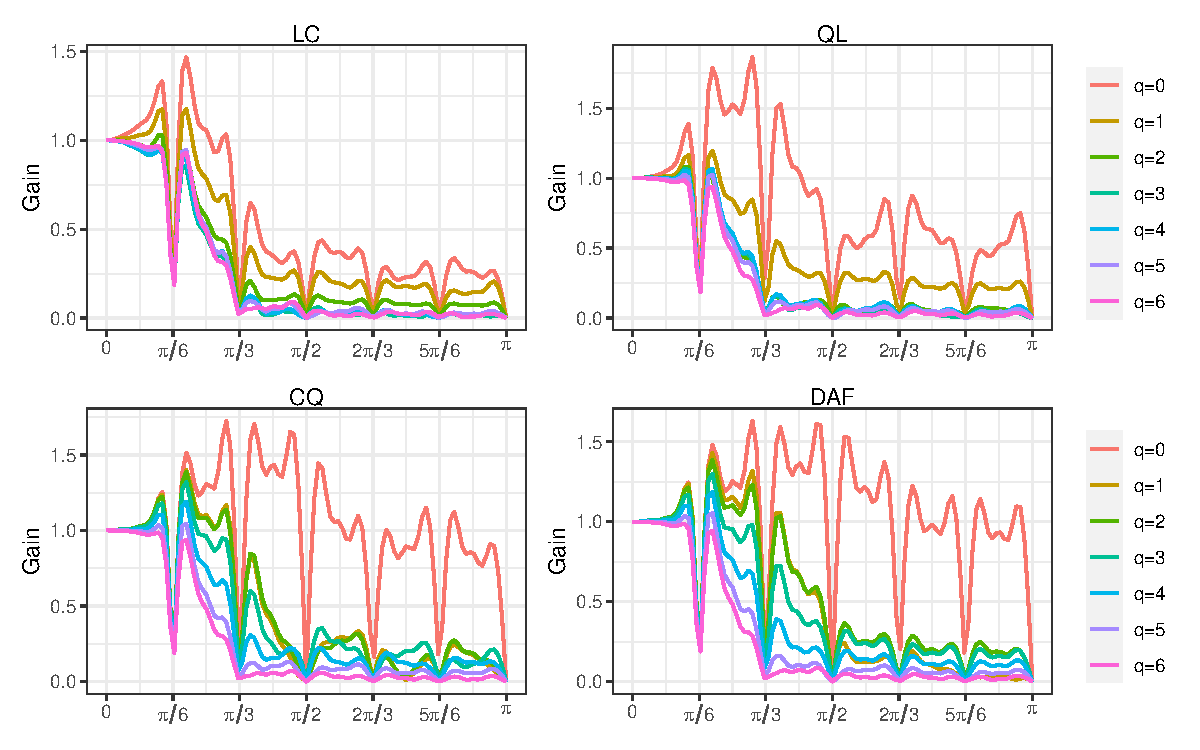
\includegraphics[width=1\linewidth]{img/gain_lp} \end{center}
\end{frame}

\begin{frame}{ex \texttt{rjd3filters} : filtres X-11}
\protect\hypertarget{ex-rjd3filters-filtres-x-11-1}{}
\begin{center}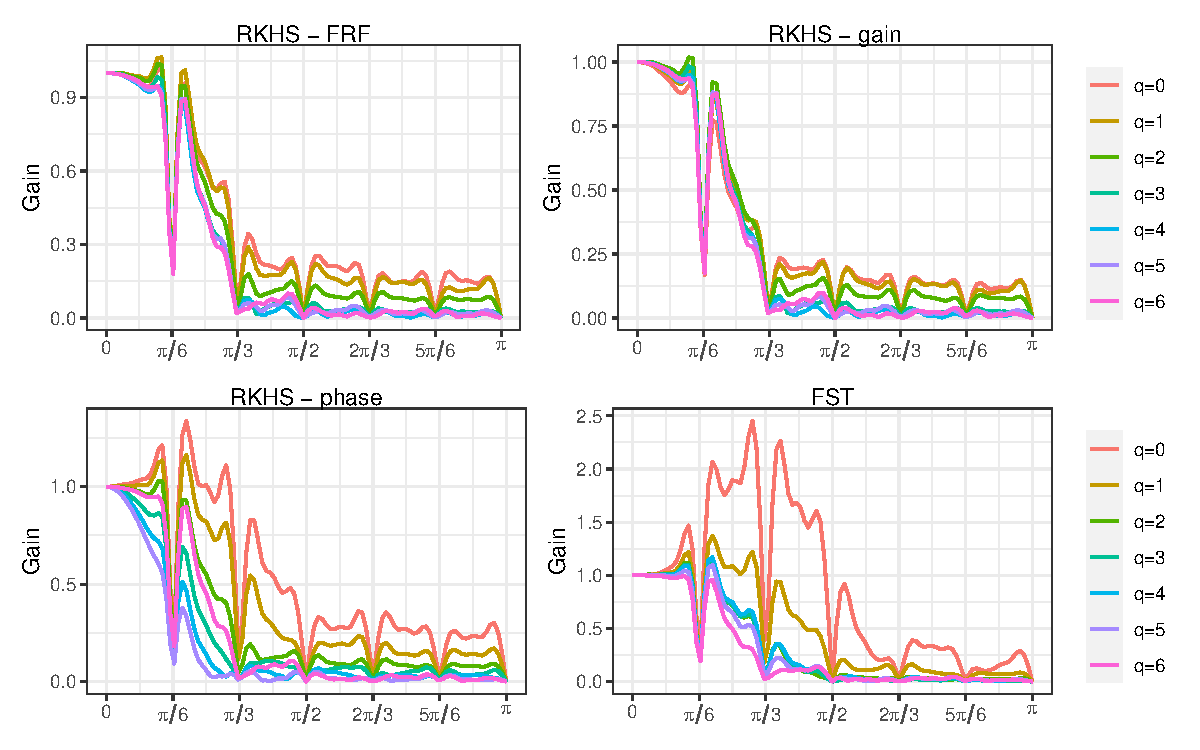
\includegraphics[width=1\linewidth]{img/gain_autres} \end{center}
\end{frame}

\end{document}
